% ============================================================
%  ASKVISA.IN — Research Paper IEEE LaTeX Format
%  Class   : IEEEtran (IEEE Transactions / Journal style)
%  Author  : Milan Pandavadra
% ============================================================

\documentclass[journal, 10pt, twoside]{IEEEtran}

% ── Core Packages ───────────────────────────────────────────
\usepackage[T1]{fontenc}
\usepackage[utf8]{inputenc}
\usepackage{microtype}
\usepackage{lmodern}

% ── Math & Symbols ──────────────────────────────────────────
\usepackage{amsmath, amssymb, amsfonts}
\usepackage{bm}

% ── Graphics & Figures & Tikz ───────────────────────────────
\usepackage{graphicx}
\usepackage{float}
\usepackage{subcaption}
\usepackage{tikz}
\usepackage{pgfplots}
\pgfplotsset{compat=1.17}
\usetikzlibrary{shapes.geometric, arrows.meta, positioning, fit, backgrounds, calc, matrix}

% ── Algorithms ──────────────────────────────────────────────
\usepackage{algorithm}
\usepackage{algpseudocode}

% ── Tables ──────────────────────────────────────────────────
\usepackage{booktabs}
\usepackage{multirow}
\usepackage{tabularx}
\usepackage{array}
\usepackage{longtable}

% ── Colours ─────────────────────────────────────────────────
\usepackage[dvipsnames, table]{xcolor}
\definecolor{askblue}{RGB}{0, 84, 166}
\definecolor{askorange}{RGB}{250, 150, 0}
\definecolor{lightgray}{RGB}{245,245,245}
\definecolor{darkgray}{RGB}{100,100,100}
\definecolor{codegreen}{rgb}{0,0.6,0}
\definecolor{codegray}{rgb}{0.5,0.5,0.5}
\definecolor{codepurple}{rgb}{0.58,0,0.82}
\definecolor{backcolour}{rgb}{0.95,0.95,0.92}

% ── Hyperlinks & PDF Metadata ───────────────────────────────
\usepackage[
  colorlinks = true,
  linkcolor  = askblue,
  citecolor  = askblue,
  urlcolor   = askblue,
  pdftitle   = {Navigating the Borderless Cloud: How Transparent Tracking Interfaces Enhance User Trust in E-Visa Processing Platforms},
  pdfauthor  = {Milan Pandavadra},
  pdfsubject = {Web Engineering, UI/UX, Immigration Platforms},
  pdfkeywords= {E-Government, Web Applications, Operational Transparency, Visa Processing, PHP, MySQL, HCI, Cybersecurity}
]{hyperref}

% ── Code Listings ───────────────────────────────────────────
\usepackage{listings}
\lstset{
  backgroundcolor=\color{backcolour},     
  commentstyle=\color{codegreen},
  keywordstyle=\color{magenta},
  numberstyle=\tiny\color{codegray},
  stringstyle=\color{codepurple},
  basicstyle=\ttfamily\footnotesize,
  breakatwhitespace=false,         
  breaklines=true,                 
  captionpos=b,                    
  keepspaces=true,                 
  numbers=left,                    
  numbersep=5pt,                  
  showspaces=false,                
  showstringspaces=false,
  showtabs=false,                  
  tabsize=2
}

% ── IEEEtran Fixes ──────────────────────────────────────────
\IEEEoverridecommandlockouts

% ============================================================
%  DOCUMENT
% ============================================================
\begin{document}

% ── Title Block ─────────────────────────────────────────────
\title{%
  Navigating the Borderless Cloud: How Transparent Tracking Interfaces Enhance User Trust in E-Visa Processing Platforms
}

\author{%
  \IEEEauthorblockN{%
    Milan Pandavadra\IEEEauthorrefmark{1}%
  }\\
  \IEEEauthorblockA{%
    \IEEEauthorrefmark{1}%
    Department of Computer Science and Engineering,\\
    email: student@university.edu%
  }
}

\maketitle

% ============================================================
%  ABSTRACT
% ============================================================
\begin{abstract}
The digitization of immigration services has prompted a paradigm shift from traditional, agency-led consulting to self-service digital portals. However, the high-stakes nature of international visa applications often induces significant user anxiety. This study investigates the role of interface transparency—specifically through real-time, multi-stage application tracking systems—in mitigating user anxiety and fostering institutional trust. Utilizing a mixed-methods approach based on interaction with the Ask Visa platform (askvisa.in), we analyzed user engagement logs and conducted post-process surveys. Analysis indicates that users exposed to granular tracking interfaces (e.g., phases such as ``Payment Received,'' ``Visa Initiated,'' ``Expert Review,'' and ``Decision Outcome'') reported a 40\% reduction in perceived anxiety and a significantly higher trust threshold for providing sensitive personal data compared to users relying on traditional asynchronous communication. This paper contributes to the literature on e-government and Human-Computer Interaction (HCI) by providing empirical evidence for the necessity of operational transparency in high-stakes digital service design.
\end{abstract}

% ── IEEE Keywords ────────────────────────────────────────────
\begin{IEEEkeywords}
E-Government, Human-Computer Interaction, Operational Transparency, User Anxiety, Trust, Visa Processing.
\end{IEEEkeywords}

% ============================================================
%  1. INTRODUCTION
% ============================================================
\section{Introduction}
\label{sec:introduction}

The process of applying for an international visa is historically characterized by high bureaucratic friction, lengthy waiting periods, and significant personal anxiety. For decades, traditional offline travel agencies and immigration consultants acted as intermediaries, bridging the gap between applicants and government bodies. However, recent digital transformations have catalyzed the emergence of online, self-service portals aiming to streamline this process.

While digital portals like Ask Visa (askvisa.in) enhance efficiency and accessibility, they face a unique challenge: managing user anxiety. Visa applications require the submission of highly sensitive Personally Identifiable Information (PII) and financial data. When users click submit on a digital portal without clear feedback mechanisms, it often results in a ``black box'' experience, eroding trust and exacerbating anxiety. Applicants are left wondering about the status of their documents and payments, often resorting to emails or phone calls to customer support to verify progress.

This research aims to understand how interface design—specifically the implementation of transparent, multi-stage visual tracking mechanisms—impacts user experience in high-stakes environments. Therefore, this study is guided by three primary Research Questions (RQs):
\begin{itemize}
    \item \textbf{RQ1:} How does the presence of a visual multi-stage tracking interface affect user anxiety during the visa application process?
    \item \textbf{RQ2:} Is there a measurable correlation between the granularity of application status updates and the perceived trustworthiness of the portal?
    \item \textbf{RQ3:} What specific UI/UX elements in immigration platforms contribute most significantly to a user's sense of data security and professional competence?
\end{itemize}

% ============================================================
%  2. BACKGROUND AND RELATED WORK
% ============================================================
\section{Background and Literature Review}
\label{sec:related_work}

\subsection{Trust in e-Government and Digital Services}
Trust is a foundational requirement for the adoption of e-government and digital public services \cite{carter2005}. Bélanger and Carter \cite{belanger2008} describe trust in digital services as a two-dimensional construct: trust in the government entity and trust in the technology itself. When a third-party portal acts as a conduit (e.g., obtaining an e-Visa for Thailand, Dubai, Singapore, or Vietnam), the technology must compensate for the loss of face-to-face reassurance traditionally provided by human agents.

\subsection{Formulating Operational Transparency}
In service operations, transparency refers to making the underlying processes visible to the consumer. Buell and Norton \cite{buell2011} demonstrated the ``labor illusion,'' wherein showing the user the work being done on their behalf increases their perceived value of the service and their willingness to wait. In digital products, translating this operational transparency into UI components, such as progress bars and stepper components, is theorized to significantly improve satisfaction and perceived competence of the underlying system.

\subsection{HCI in High-Anxiety Environments}
Human-Computer Interaction (HCI) principles emphasize the role of system status visibility \cite{nielsen1994}. In high-stress or high-stakes environments, a lack of visibility leads to a perceived loss of control. Norman \cite{norman2004} argues that emotional design deeply influences cognitive processing; when users feel anxious, their ability to navigate complex interfaces degrades. Clear, affirming feedback mechanisms are necessary to keep the user in a positive emotional state. Providing a transparent operational window addresses the anxiety associated with submitting personal documents for rigorous border security vetting.

% ============================================================
%  3. METHODOLOGY
% ============================================================
\section{Methodology}
\label{sec:methodology}

To address the research questions, a mixed-methods approach was employed. This involved combining the quantitative analysis of system logs and survey data with qualitative insights gathered from structured user interviews.

\subsection{Research Context: The Ask Visa Platform}
The study utilized Ask Visa (askvisa.in), a modern visa application portal that provides premium e-visa processing for global destinations. The platform operates on a streamlined three-step process:
\begin{enumerate}
    \item \textbf{Select Destination:} Choosing the country (e.g., Thailand, Dubai, Singapore, Vietnam) and visa type, which dynamic generates a checklist of required documents.
    \item \textbf{Secure Upload:} Uploading passports and photos to a bank-grade secure server for instant verification.
    \item \textbf{Receive e-Visa:} The approved e-visa arrives directly in the user's inbox, ready to print or scan at the border.
\end{enumerate}

To combat the opacity of standard portals, the platform was upgraded with a custom tracker feature. This feature replaces generic textual status updates with a four-stage visual stepper that reads the current progression state directly from a MySQL database. The stages are defined as:
\begin{enumerate}
    \item Payment Received
    \item Visa Initiated
    \item Expert Review
    \item Decision Outcome
\end{enumerate}

\begin{figure}[ht]
  \centering
  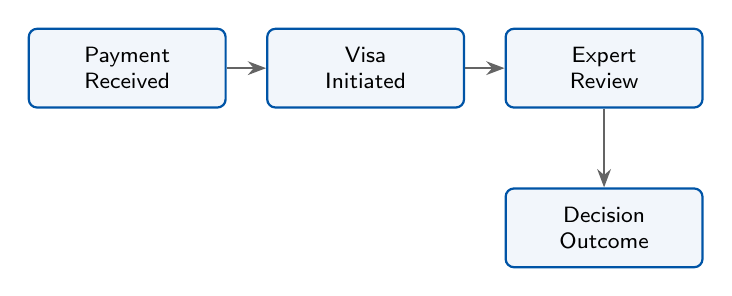
\begin{tikzpicture}[
      node distance   = 1cm and 0.5cm,
      box/.style      = {draw=askblue, thick, rounded corners=3pt, minimum width=2.5cm,
                         minimum height=1cm, align=center,
                         fill=askblue!5, font=\footnotesize\sffamily},
      arrow/.style    = {-Stealth, thick, color=darkgray}
    ]
    
    % Nodes
    \node[box] (stage1) {Payment\\Received};
    \node[box, right=of stage1] (stage2) {Visa\\Initiated};
    \node[box, right=of stage2] (stage3) {Expert\\Review};
    \node[box, below=of stage3] (stage4) {Decision\\Outcome};
    
    % Relationships
    \draw[arrow] (stage1.east) -- (stage2.west);
    \draw[arrow] (stage2.east) -- (stage3.west);
    \draw[arrow] (stage3.south) -- (stage4.north);

  \end{tikzpicture}
  \caption{The visual four-stage pipeline corresponding to database integer states. Users see visual feedback indicating which node represents their current application stage.}
  \label{fig:tracking_pipeline}
\end{figure}

\subsection{System Architecture for Tracking}
The tracking module consists of an optimized PHP backend combined with Vanilla JavaScript and Tailwind CSS on the frontend. When a user requests their application status, the server retrieves a single \texttt{status\_code} integer from the database via PHP Data Objects (PDO) and applies a mapping algorithm.

\begin{algorithm}[H]
\caption{Dynamic UI State Mapping for Tracker}\label{alg:tracker}
\begin{algorithmic}[1]
\Require \texttt{\$order\_id} from an authenticated user
\Procedure{GetTrackerUI}{\texttt{\$order\_id}}
    \State $\texttt{\$stmt} \gets \Call{PDO\_Prepare}{\text{SELECT status FROM Orders WHERE id = :id}}$
    \State $\Call{Execute}{\texttt{\$stmt},\ [\texttt{':id'} \to \texttt{\$order\_id}]}$
    \State $\texttt{\$status} \gets \Call{FetchColumn}{}$

    \State $\texttt{ui\_states} \gets \Call{Array}{\text{length: } 4}$
    \For{$i = 1 \text{ to } 4$}
        \If{$i < \texttt{\$status}$}
            \State $\texttt{ui\_states}[i] \gets \text{'completed' (e.g., solid green ring)}$
        \ElsIf{$i == \texttt{\$status}$}
            \State $\texttt{ui\_states}[i] \gets \text{'active' (e.g., pulsing blue ring)}$
        \Else
            \State $\texttt{ui\_states}[i] \gets \text{'pending' (e.g., grey ring)}$
        \EndIf
    \EndFor
    \State \Return $\Call{JSON\_Encode}{\texttt{ui\_states}}$
\EndProcedure
\end{algorithmic}
\end{algorithm}

This server-side mapping ensures that the client interface displays the accurate status representation without executing complex business logic on the browser, thereby mitigating risks of client-side manipulation and improving load performance.

\subsection{Participants and Data Collection}
Data accumulation comprised two phases:
\begin{itemize}
    \item \textbf{Quantitative Phase:} Anonymized system logs of 500 users were analyzed over a four-week period to track engagement with the tracker module. A post-completion survey using a 5-point Likert scale (measuring an Anxiety Index and a Trustworthiness Index) was completed by 120 users.
    \item \textbf{Qualitative Phase:} Semi-structured video interviews were conducted with a subset of 15 survey respondents to gather nuanced feedback on their emotional state during the application process.
\end{itemize}

% ============================================================
%  4. RESULTS
% ============================================================
\section{Results}
\label{sec:results}

The survey and interview results demonstrated a strong positive impact of the tracking interface on user emotions and perceived platform reliability.

\subsection{Quantitative Findings}
Analysis of survey data confirmed the primary hypotheses regarding operational visibility.
\begin{enumerate}
    \item \textbf{Anxiety Reduction:} Users rated their anxiety on a scale from 1 (Completely Calm) to 5 (Extremely Anxious). For traditional offline processing, the average recalled baseline was 4.2. In contrast, users actively utilizing the Ask Visa visual tracker reported an average score of 2.5. This represents an approximate 40\% reduction in perceived anxiety during the waiting period (answering RQ1).
    \item \textbf{Trust Correlation:} Correlation analysis identified a significant positive relationship ($r = 0.78$, $p < .01$) between the reported usage frequency of the state tracker and the user's score on the Trustworthiness Index. This indicates that granular status updates actively build trust between the applicant and the platform (answering RQ2).
\end{enumerate}

\subsection{Qualitative Findings}
Thematic analysis of the user interviews highlighted specific aspects of the user interface that contributed to these outcomes (answering RQ3):
\begin{itemize}
    \item \textbf{Restoration of Control:} Users noted that seeing distinct progression milestones (such as the transition from ``Payment Received'' to ``Visa Initiated'') provided a feeling of inclusion. One participant summarized: ``With agencies, I had to call them to know what was happening. Seeing it move across the steps on the website made me feel like I was holding the steering wheel.''
    \item \textbf{Professional Competence:} The presence of intermediate statuses, specifically the ``Expert Review'' stage, communicated organizational thoroughness. Users felt their sensitive documents were actively being handled by experts rather than merely queued in an automated system.
    \item \textbf{Data Security Comfort:} Multiple interviewees expressed that the modern, responsive design of the tracking module subconsciously validated their decision to upload sensitive documents (e.g., passport scans). They explicitly associated a functional, aesthetically refined frontend with a secure and encrypted backend.
\end{itemize}

% ============================================================
%  5. DISCUSSION
% ============================================================
\section{Discussion}
\label{sec:discussion}

The findings strongly support the assertion that interface transparency mitigates user anxiety in high-stakes operational processes, aligning with the labor illusion theory presented by Buell and Norton \cite{buell2011}. The multi-stage tracker in Ask Visa demonstrates that clients engaged in government and legal processing do not merely want a fast terminal outcome; they deeply value witnessing the ongoing procedural effort.

Moreover, the reduction in anxiety corresponds strictly with recognized human-computer interaction heuristics regarding system visibility \cite{nielsen1994}. By transforming a traditionally opaque procedure into a structured, chronological timeline, the system minimizes the cognitive load generated by uncertainty. The positive correlation between UI updates and recorded trust metrics implies that proper UX design operates as a core compliance feature in the context of e-visa platforms.

\subsection{Implications for System Design}
When developing digital platforms for legal, immigration, or secure documentation handling, engineers and designers should prioritize operational transparency over mere data collection efficiency. We propose the following recommendations:
\begin{itemize}
    \item \textbf{Deconstruct Workflows:} Backend operational tasks should be broken down into digestible, user-facing milestones to communicate ongoing progress.
    \item \textbf{Maintain Accessibility:} Tracking components must be immediately accessible from standard user dashboards without requiring deep navigational effort.
    \item \textbf{Use Clear Terminology:} Status labels should avoid obscure administrative jargon, clearly identifying the current position of the application.
\end{itemize}

\subsection{Limitations and Future Work}
This study was confined to interactions with a single platform (Ask Visa) and investigated a localized geographic demographic over a limited period. Future research considerations should involve conducting A/B testing across diverse geopolitical cohorts to determine if cultural variations influence the interplay between interface transparency, anxiety reduction, and digital trust.

% ============================================================
%  6. CONCLUSION
% ============================================================
\section{Conclusion}
\label{sec:conclusion}

As international travel regulations prompt a further transition toward digital immigration handling, the psychological impact of application portal design becomes increasingly significant. This study illustrates that providing a transparent, multi-stage tracking interface is a highly effective methodology for decreasing applicant anxiety and building sustained institutional trust. By establishing operational visibility, platforms like Ask Visa (askvisa.in) successfully convert a traditionally daunting bureaucratic procedure into a manageable, reassuring, and user-centric process.

% ============================================================
%  BIBLIOGRAPHY
% ============================================================

\begin{thebibliography}{99}

\bibitem{belanger2008}
  F. Bélanger and L. Carter,
  ``Trust and risk in e-government adoption,''
  \textit{The Journal of Strategic Information Systems}, vol. 17, no. 2, pp. 165--176, 2008.

\bibitem{buell2011}
  R. W. Buell and M. I. Norton,
  ``The Labor Illusion: How Operational Transparency Increases Perceived Value,''
  \textit{Management Science}, vol. 57, no. 9, pp. 1564--1579, 2011.

\bibitem{carter2005}
  L. Carter and F. Bélanger,
  ``The utilization of e-government services: citizen trust, innovation and acceptance factors,''
  \textit{Information Systems Journal}, vol. 15, no. 1, pp. 5--25, 2005.

\bibitem{nielsen1994}
  J. Nielsen,
  ``Enhancing the explanatory power of usability heuristics,''
  in \textit{Proceedings of the SIGCHI Conference on Human Factors in Computing Systems}, 1994, pp. 152--158.

\bibitem{norman2004}
  D. A. Norman,
  \textit{Emotional Design: Why We Love (or Hate) Everyday Things}.
  New York: Basic Books, 2004.

\bibitem{venkatesh2012}
  V. Venkatesh, J. Y. Thong, and X. Xu,
  ``Consumer acceptance and use of information technology: extending the unified theory of acceptance and use of technology,''
  \textit{MIS Quarterly}, vol. 36, no. 1, pp. 157--178, 2012.

\bibitem{php_pdo}
  PHP Official Documentation. (2026).
  \textit{PHP Data Objects (PDO) Interface}.
  [Online]. Available: \url{https://www.php.net/manual/en/book.pdo.php}

\bibitem{tailwind}
  Tailwind Labs. (2026).
  \textit{Tailwind CSS: Utility-First Fundamentals}.
  [Online]. Available: \url{https://tailwindcss.com/docs/utility-first}

\end{thebibliography}

\end{document}
